\documentclass[11pt,a4paper]{article}

\usepackage[margin=2.2cm]{geometry}
\usepackage{graphicx}
\usepackage{hyperref}
\usepackage{xcolor}
\usepackage{booktabs}
\usepackage{tabularx}
\usepackage{enumitem}
\usepackage{fancyhdr}
\usepackage{titlesec}
\usepackage{listings}
\usepackage{caption}
\usepackage{fontenc}
\usepackage[utf8]{inputenc}
\usepackage{parskip}

% ── Colors (Metaflow palette) ──
\definecolor{mfpurple}{HTML}{7B68AE}
\definecolor{mfblue}{HTML}{1A56DB}
\definecolor{mfgreen}{HTML}{4AA86B}
\definecolor{mfred}{HTML}{E85757}
\definecolor{mfbg}{HTML}{F0ECE3}
\definecolor{mfgray}{HTML}{6B6B6B}
\definecolor{codebg}{HTML}{2D2D2D}
\definecolor{codetext}{HTML}{E0E0E0}

% ── Typography ──
\hypersetup{
    colorlinks=true,
    linkcolor=mfblue,
    urlcolor=mfblue,
    citecolor=mfblue,
}

\titleformat{\section}{\Large\bfseries\color{mfpurple}}{}{0em}{}[\vspace{-0.5em}\color{mfpurple}\rule{\textwidth}{0.5pt}]
\titleformat{\subsection}{\large\bfseries}{}{0em}{}
\titleformat{\subsubsection}{\normalsize\bfseries\color{mfgray}}{}{0em}{}

% ── Code style ──
\lstset{
    backgroundcolor=\color{codebg},
    basicstyle=\ttfamily\small\color{codetext},
    breaklines=true,
    frame=single,
    rulecolor=\color{codebg},
    xleftmargin=1em,
    framexleftmargin=0.5em,
    numbers=none,
    showstringspaces=false,
    tabsize=4,
    keywordstyle=\color{mfgreen},
    commentstyle=\color{mfgray},
    stringstyle=\color{mfred},
}

% ── Header ──
\pagestyle{fancy}
\fancyhf{}
\fancyhead[L]{\small\color{mfgray}GSoC 2026 Proposal}
\fancyhead[R]{\small\color{mfgray}Agent-Friendly Metaflow Client}
\fancyfoot[C]{\small\color{mfgray}\thepage}
\renewcommand{\headrulewidth}{0.4pt}

\begin{document}

% ═══════════════════════════════════════════════════════════
% TITLE PAGE
% ═══════════════════════════════════════════════════════════

\begin{titlepage}
\begin{center}
\vspace*{1.5cm}

{\Huge\bfseries\color{mfpurple} Agent-Friendly\\[0.3em] Metaflow Client}

\vspace{0.8em}

{\Large Analyzing and Addressing Client API Inefficiencies}

\vspace{1.5em}

{\large GSoC 2026 Proposal}

\vspace{2em}

\begin{tabular}{rl}
\textbf{Applicant:} & Gennaro Francesco Landi \\
\textbf{University:} & ETH Zurich, MSc Computer Science \\
\textbf{Mentor:} & Valay Dave, Outerbounds \\
\textbf{Project:} & Large (350 hours) \\
\textbf{Date:} & \today \\
\end{tabular}

\vspace{2em}

\colorbox{mfbg}{%
\begin{minipage}{0.85\textwidth}
\centering\vspace{0.6em}
\textbf{Verified:} We pointed an LLM agent at a ForeachFlow and asked it to find failed tasks. It wrote 6 lines of Client API code that triggered \textbf{57 HTTP calls} (51 artifact fetches to unpickle booleans). The metadata service answers the same question in \textbf{4 calls} via \texttt{filter\_tasks\_by\_metadata}. Full API trace attached.
\vspace{0.6em}
\end{minipage}%
}

\vfill
{\small\color{mfgray} \href{https://drive.google.com/file/d/1kOcsjZq4CIPGR2IsXiEggBKzrgb08ME4/view?usp=sharing}{Presentation (Google Drive)} and documentation attached.}
\end{center}
\end{titlepage}

% ═══════════════════════════════════════════════════════════
\section{About Me}
% ═══════════════════════════════════════════════════════════

\textbf{Name:} Gennaro Francesco Landi \hfill \textbf{GitHub:} \href{https://github.com/landigf}{github.com/landigf}

\textbf{University:} ETH Zurich, MSc Computer Science (1st year)

\subsection{Technical Background}

My interest is in how AI agent workloads stress infrastructure designed for humans. The gap between ``human clicks through a UI'' and ``agent issues 200 API calls in a loop'' is where things break. That's exactly what this project is about.

\begin{itemize}[nosep]
    \item \textbf{Python}: library internals, monkeypatching for instrumentation, profiling call chains
    \item \textbf{REST APIs}: built and profiled database-backed service layers
    \item \textbf{Open source}: \href{https://github.com/landigf}{github.com/landigf}
\end{itemize}

\subsection{Recent: StartHack 2026 --- Winner (Internal Challenge)}

I used Metaflow at StartHack, a 36-hour hackathon, but \textit{not} for its typical ML workflow use case. Our team needed a decision-process pipeline with auditing, verification, and consistency guarantees. I reached for Metaflow because (1) we needed a DAG to enforce coherence across decision stages, (2) we needed something deployable to the cloud fast, and (3) Metaflow's Azure integration made that trivial. We won the internal challenge and pitched to investors in the finals.

What this showed: Metaflow's value extends beyond ML --- the DAG visualization, repeatable execution, and cloud deployment worked for a compliance/decision use case, all built in under 36 hours.

\begin{figure}[h!]
\centering
\begin{minipage}[t]{0.45\textwidth}
\centering
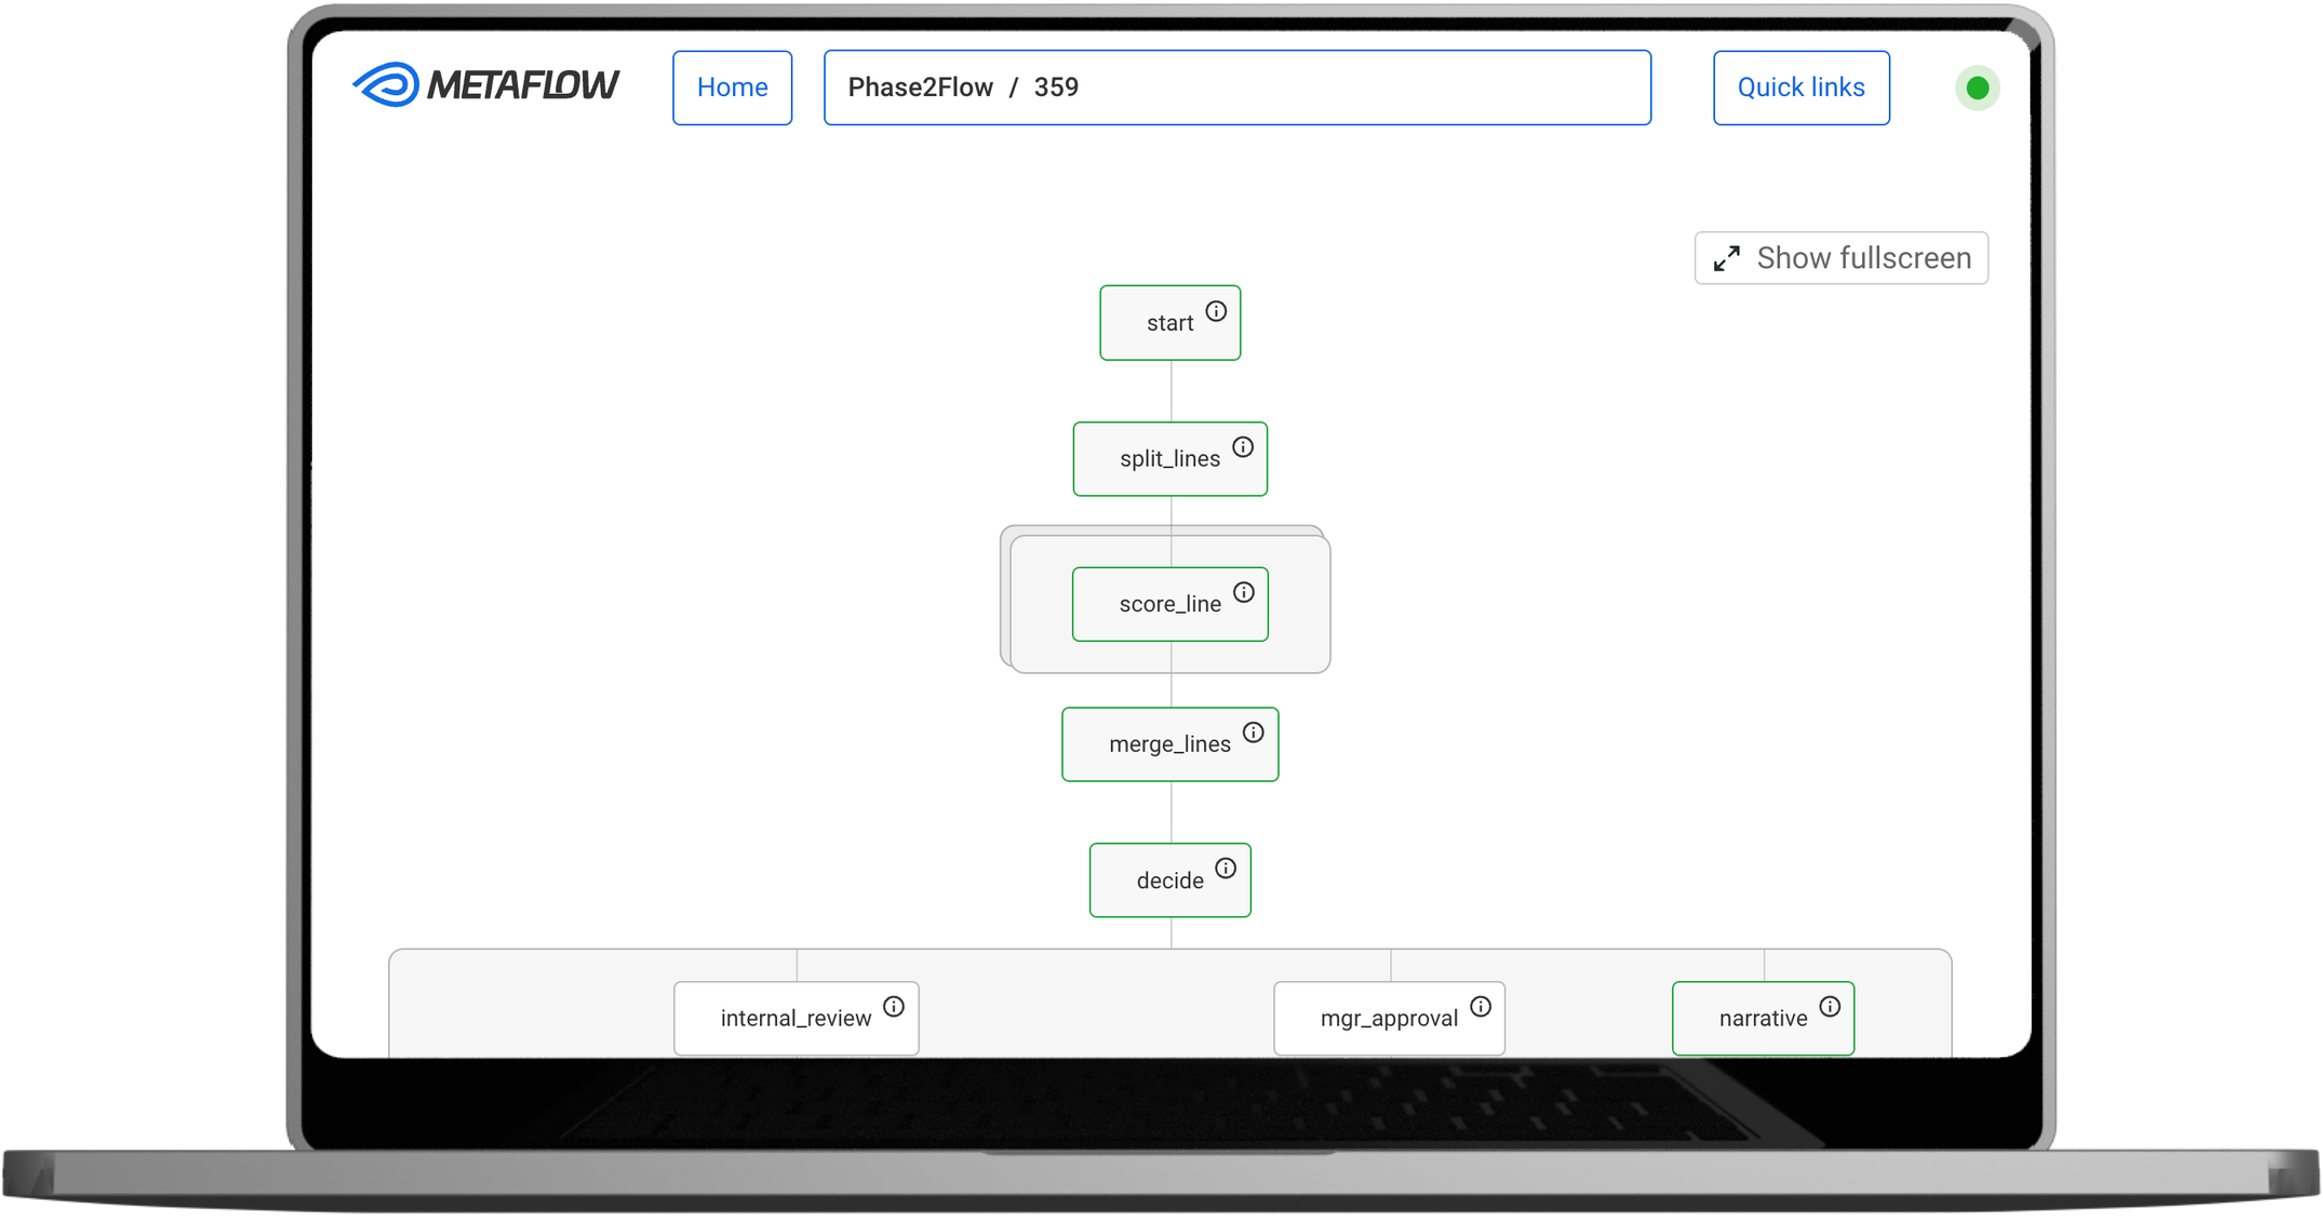
\includegraphics[width=\textwidth]{pitch_metaflow.png}
\caption*{\small\color{mfgray} Metaflow UI showing the procurement pipeline DAG.}
\end{minipage}
\hfill
\begin{minipage}[t]{0.50\textwidth}
\centering
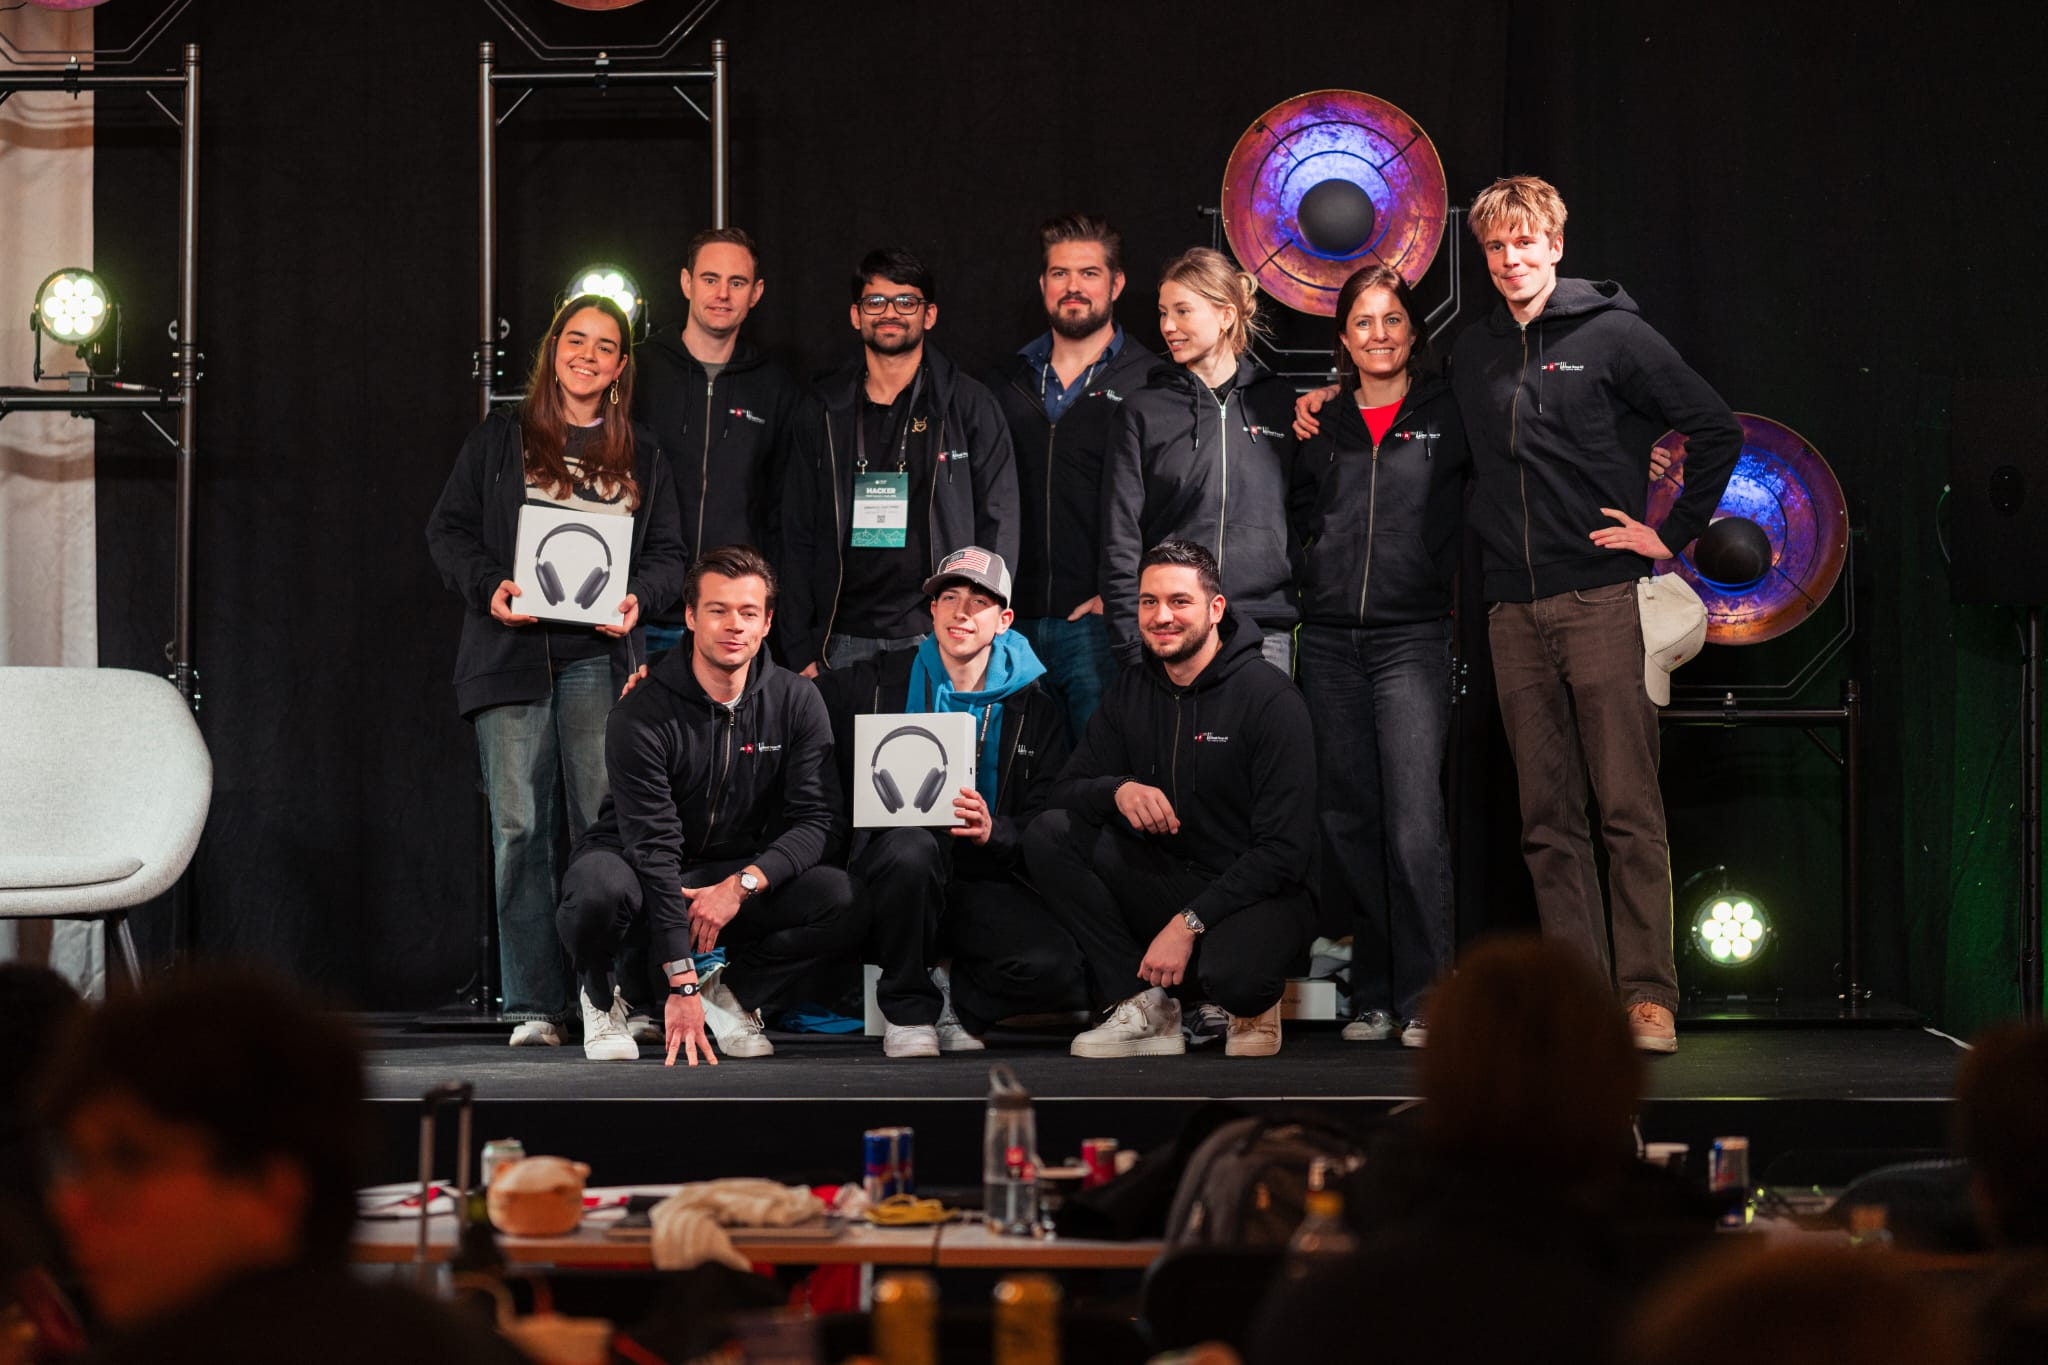
\includegraphics[width=\textwidth]{starthack_win.jpg}
\caption*{\small\color{mfgray} StartHack 2026 winning ceremony.}
\end{minipage}
\end{figure}

\subsection{Why This Project}

I pointed an LLM agent at a Metaflow flow and asked it to find a failed task. It wrote correct code. That code made 57 HTTP requests. The UI Backend answers the same question in 2. Both read the same database. That gap shouldn't exist.

I dug into the codebase to understand why it does. This proposal is the result --- not a restatement of the project description, but findings from actually instrumenting the code and running benchmarks.


% ═══════════════════════════════════════════════════════════
\section{Project Description}
% ═══════════════════════════════════════════════════════════

\subsection{The Problem}

I asked an LLM agent a simple question: ``which tasks failed in my latest ForeachFlow run?'' It wrote this code --- unprompted:

\begin{lstlisting}[language=Python]
from metaflow import Flow
flow = Flow('ForeachFlow')
latest_run = flow.latest_run
for step in latest_run:
    for task in step:
        if not task.successful:
            print(task.pathspec)
\end{lstlisting}

Correct answer. But here's the cost:

\begin{center}
\begin{tabular}{lrrr}
\toprule
& \textbf{HTTP Calls} & \textbf{Datastore Reads} & \textbf{Time} \\
\midrule
What the agent's code costs & 57 & 50 & 2,074ms \\
\bottomrule
\end{tabular}
\end{center}

51 of those 57 calls are \texttt{GET .../artifacts/\_success} --- one per task, each hitting the datastore to unpickle a boolean. This isn't the agent being dumb. This is the \textbf{only way} to check task success with the current Client API. There is no \texttt{run.failed\_tasks()}. The full HTTP trace is in the attached \texttt{llm\_api\_trace.json}.

\subsection{Three Discoveries}

I set up the full dev stack, monkeypatched \texttt{ServiceMetadataProvider.\_request} to count every HTTP call, and traced all six use cases from the project description. Three things came out that changed the whole approach:

\subsubsection{The metadata service already knows which tasks failed}

Since v2.5.0, this works:

\begin{lstlisting}[language=Python]
ServiceMetadataProvider.filter_tasks_by_metadata(
    "ForeachFlow", "8", "process", "attempt_ok", "False"
)
# Returns: ["ForeachFlow/8/process/126"]  -- one call, done.
\end{lstlisting}

The Metaflow runtime writes \texttt{attempt\_ok} to the metadata table when a task finishes. This queries it directly. One call. No artifacts, no datastore, no unpickling.

\subsubsection{The DB layer already supports pagination --- it's just not wired up}

\texttt{find\_records()} in \texttt{postgres\_async\_db.py} takes \texttt{limit}, \texttt{offset}, and \texttt{order} parameters. The HTTP endpoints don't pass them through. Wiring \texttt{?\_limit=10\&\_order=-ts\_epoch} is $\sim$15 lines per endpoint. The plumbing exists, the faucet is just turned off.

\subsubsection{Task status is simpler than it looks}

The UI Backend computes status with 300 lines of SQL. Most of it handles edge cases. The core logic:

\begin{lstlisting}[language=SQL]
CASE
  WHEN attempt_ok = 'True'  THEN 'completed'
  WHEN attempt_ok = 'False' THEN 'failed'
  ELSE 'running'
END
\end{lstlisting}

Covers 90\% of cases. The other 10\% (stale heartbeats, old runs without activity) can come later.

\subsection{Three-Path Benchmark}

To make this concrete, I built a Metaflow flow that benchmarks itself. Three parallel branches, same question, same database. The DAG is visible in the Metaflow UI:

\begin{center}
\begin{tabular}{llrrl}
\toprule
\textbf{Path} & \textbf{Approach} & \textbf{Calls} & \textbf{Time} & \textbf{Infrastructure} \\
\midrule
\textcolor{mfred}{A: Naive} & Iterate tasks, fetch \texttt{\_success} per task & 56 & 3,800ms & Metadata service \\
\textcolor{mfgreen}{C: Smart} & \texttt{filter\_tasks\_by\_metadata} & 4 & 349ms & Metadata service \\
\textcolor{mfblue}{B: UI Backend} & Rich query, status in response & 2 & 35ms & + UI Backend \\
\bottomrule
\end{tabular}
\end{center}

Same failed task, every time. Path C is the target: \textbf{8.6$\times$ faster}, works everywhere, zero new infrastructure. UI Backend is a bonus when available, not a dependency.

\begin{figure}[h!]
\centering
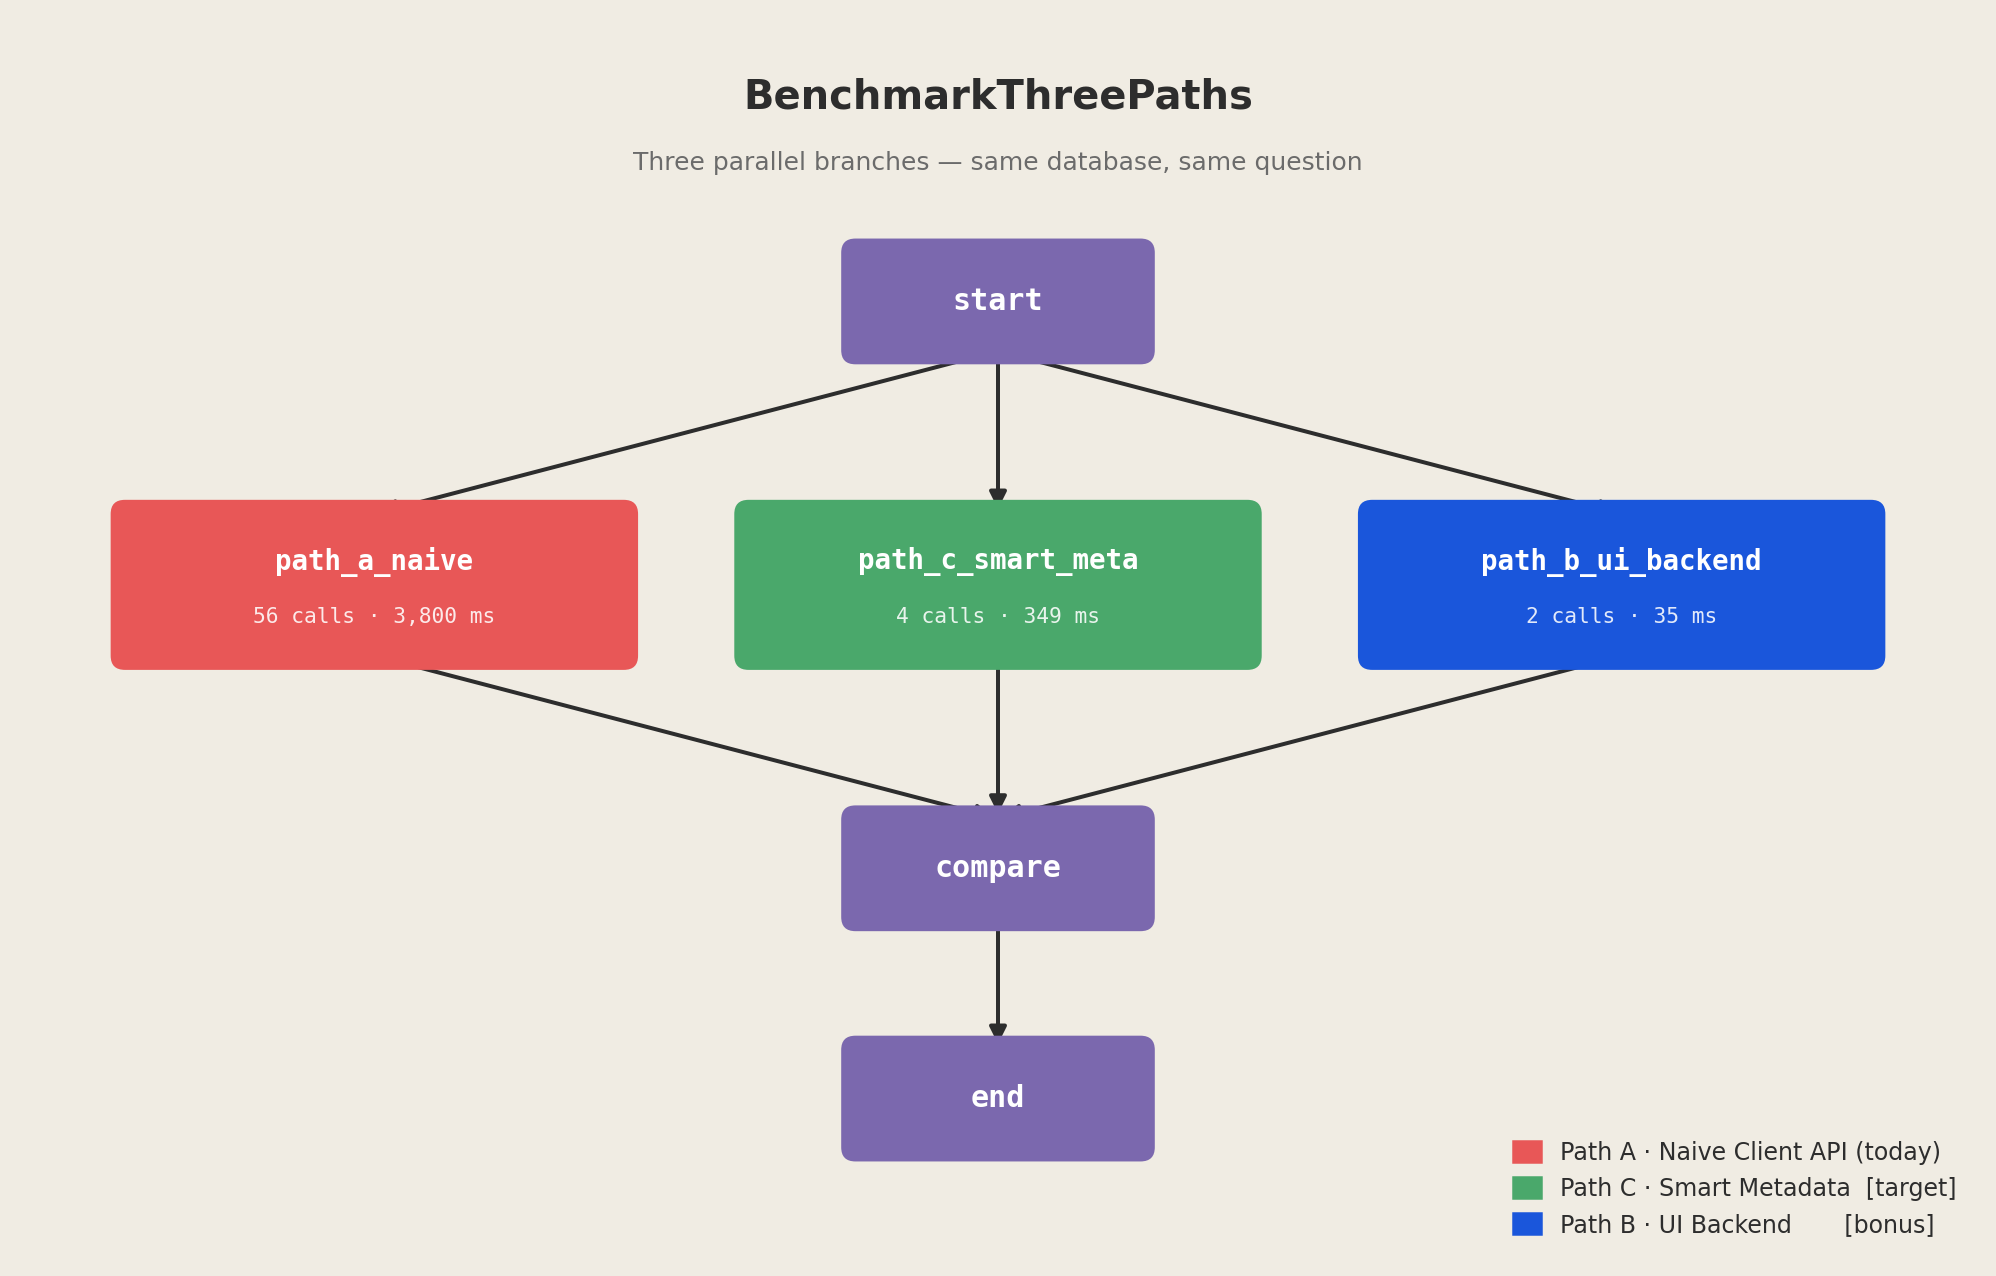
\includegraphics[width=0.92\textwidth]{benchmark_dag.png}
\caption*{\small\color{mfgray} BenchmarkThreePaths — three parallel branches, one joined result. Colours match the benchmark table above.}
\end{figure}

\subsection{Full Audit: All 6 Use Cases}

\begin{center}
\begin{tabular}{clrrl}
\toprule
\textbf{UC} & \textbf{Use Case} & \textbf{Client API} & \textbf{Smart Path} & \textbf{Speedup} \\
\midrule
1 & List runs by status & 4 calls & 1 call & 6.7$\times$ \\
2 & Filter runs by time range & 2 calls & 1 call & 1.5$\times$ \\
3 & Find failed tasks + errors & 57 calls & 5 calls & \textbf{19.1$\times$} \\
4 & Artifact metadata (no data load) & 5 calls & 4 calls & $\sim$same \\
5 & Bounded log output & 6 calls & 4 calls & $\sim$same \\
6 & Cross-run artifact search & 8 calls & 5 calls & 1.8$\times$ \\
\midrule
& \textbf{Total} & \textbf{82 calls} & \textbf{20 calls} & \textbf{4.1$\times$} \\
\bottomrule
\end{tabular}
\end{center}

UC3 dominates --- 70\% of all calls come from checking task status. UC4 and UC5 are a different problem: not too many calls, but \textbf{too much data}. \texttt{task.stdout} dumps 50MB when you need 10 lines. There's no ``give me just the artifact names'' without iterating everything. The fix for those is bounded access, not fewer calls.


% ═══════════════════════════════════════════════════════════
\section{Technical Approach}
% ═══════════════════════════════════════════════════════════

\subsection{Architecture: Three Layers}

\begin{center}
\renewcommand{\arraystretch}{1.6}
\begin{tabular}{@{}p{1.8cm}p{3.4cm}p{9.2cm}@{}}
\toprule
& \textbf{What} & \textbf{Effect} \\
\midrule
\colorbox{mfgreen}{\color{white}\small\bfseries Layer 1}
  & Extension Package
  & Smart functions using \texttt{filter\_tasks\_by\_metadata} + bounded iteration.
    \textcolor{mfgreen}{No core changes. Works on service $\geq$ 2.5.0.} \\
\colorbox{mfpurple}{\color{white}\small\bfseries Layer 2}
  & Metadata Service
  & Add \texttt{\_limit}, \texttt{\_order} to endpoints (DB already supports it).
    \textcolor{mfpurple}{$\sim$150 lines. Benefits everyone, not just agents.} \\
\colorbox{mfblue}{\color{white}\small\bfseries Layer 3}
  & Client API
  & \texttt{ServiceMetadataProvider}: auto-use new query params (version-gated).
    \textcolor{mfblue}{Transparent speedup. Existing code gets faster.} \\
\bottomrule
\end{tabular}
\renewcommand{\arraystretch}{1}
\end{center}

\subsection{Extension Package: \texttt{metaflow-agent-client}}

Uses the \texttt{metaflow\_extensions} mechanism (no core changes needed):

\begin{lstlisting}[language=Python]
from metaflow_extensions.agent_client import find_failures, get_recent_runs

# 4 HTTP calls instead of 56
result = find_failures("ForeachFlow/8")
# {"failures": ["ForeachFlow/8/process/126"], "total_tasks": 50}

# Bounded listing instead of fetching all history
recent = get_recent_runs("ForeachFlow", limit=5, status="failed")
\end{lstlisting}

Six utility functions, each with internal routing:
\begin{itemize}[nosep]
    \item \texttt{find\_failures()} --- uses \texttt{filter\_tasks\_by\_metadata("attempt\_ok", "False")}
    \item \texttt{get\_recent\_runs()} --- bounded listing with optional status filter
    \item \texttt{batch\_run\_status()} --- batch status for recent runs
    \item \texttt{run\_summary()} --- structured overview of steps, tasks, failures
    \item \texttt{tail\_logs()} --- last N lines of a task's stdout/stderr
    \item \texttt{get\_runs\_since()} --- time-filtered listing
\end{itemize}

\subsection{Metadata Service Changes ($\sim$150 lines)}

\begin{center}
\begin{tabular}{lrl}
\toprule
\textbf{Change} & \textbf{Lines} & \textbf{What it enables} \\
\midrule
Add \texttt{\_limit} to listing endpoints & $\sim$15 & ``Last 5 runs'' without fetching all \\
Add \texttt{\_order} to listing endpoints & $\sim$15 & Sort by timestamp, run number \\
Simplified status via \texttt{attempt\_ok} & $\sim$40 & Task status without artifact fetching \\
Cross-task artifact listing & $\sim$40 & Artifact metadata across tasks in one call \\
Bounded log endpoint & $\sim$40 & Last N lines, no full download \\
\bottomrule
\end{tabular}
\end{center}

All changes wire to existing \texttt{find\_records()} infrastructure. The DB layer already supports these parameters.

\subsection{ServiceMetadataProvider Enhancement}

Follows the established version-gating pattern (same as \texttt{\_supports\_attempt\_gets} at \texttt{service.py:260}):

\begin{lstlisting}[language=Python]
if cls._supports_query_params is None:
    version = cls._version(None)
    cls._supports_query_params = (
        version is not None
        and version_parse(version) >= version_parse("X.Y.Z")
    )
# When True: append ?_limit=N&_order=-ts_epoch to listing URLs
# When False: current behavior (fetch all, filter client-side)
\end{lstlisting}

\subsection{Backward Compatibility}

\begin{itemize}[nosep]
    \item \textbf{Old client + new service}: Old clients don't send query params. Service returns all results. Safe.
    \item \textbf{New client + old service}: Version check detects old service, skips query params. Safe.
    \item \textbf{No UI Backend}: All functions have fallback paths. Slower, but correct.
    \item \textbf{Existing code}: \texttt{Flow()}, \texttt{Run()}, \texttt{Task()} behavior unchanged.
\end{itemize}


% ═══════════════════════════════════════════════════════════
\section{Timeline}
% ═══════════════════════════════════════════════════════════

\begin{tabularx}{\textwidth}{@{}lXrl@{}}
\toprule
\textbf{Phase} & \textbf{Goal} & \textbf{h} & \textbf{Milestone} \\
\midrule
1 (Wk 1--4)   & Extension package: 6 utility functions, unit + integration tests & 90 & Midterm checkpoint \\
2 (Wk 5--8)   & Metadata service \texttt{\_limit}/\texttt{\_order} + provider version-gating & 90 & Core changes ready \\
3 (Wk 9--12)  & Agent simulation (5 scenarios), MCP tool schemas & 90 & End-to-end validated \\
4 (Wk 13--16) & User + agent docs, PR prep per CONTRIBUTING.md, final report & 80 & Submitted \\
\bottomrule
\end{tabularx}

\textbf{Midterm checkpoint (Week 4):} Working extension package with 6 functions, all tested, benchmark showing improvement over the naive path. Each phase delivers standalone value --- Phase 1 alone is a complete, usable deliverable.

\textbf{Risks:} Core Runtime changes require pre-approved issues per CONTRIBUTING.md --- Phase 1 (extension package) requires no core changes and delivers full value independently. Status SQL complexity is mitigated by using the simplified \texttt{attempt\_ok} check (3 lines, 90\% coverage). Two-repo coordination is handled via version-gated detection.


% ═══════════════════════════════════════════════════════════
\section{Commitments \& Disclosure}
% ═══════════════════════════════════════════════════════════

\textbf{Availability:} 22+ hours/week (350h $\div$ 16 weeks). No other employment during GSoC. Exam periods and vacations will be disclosed to the mentor in advance.

\textbf{AI disclosure:} AI tools were used for codebase exploration, benchmark scaffolding, and document drafting. All code, analysis, and architectural decisions are my own. I can explain every line and design choice independently.


\end{document}
